\documentclass{article}
\usepackage{graphicx}

\begin{document}

\begin{titlepage}
\title{ECS189G Homework 1 Report}
\author{Goh Chang Kang, Charles 916751838, \\
Yang Minxing 916751773, Chen Jieyi Chloe 999823783}

\date{October 15, 2018}
\maketitle
\end{titlepage}


\section{Problem A}
The predict.usrData() function was extended by adding a new measure of location argument that receives a function. This function will then operate on all the elements, instead of just have mean as the default. 
\begin{verbatim}
predict.usrData <- function (origData, newData, newItem, k, wtcovs = NULL, 
wtcats = NULL, locMeasure = mean ) 
{
  traincovs <- !is.null(origData$usrCovs)
  newcovs <- !is.null(newData$cvrs)
  if (!(traincovs + newcovs %in% c(0, 2))) 
    stop("mismatch in having/not having covars, orig and new data")
  traincats <- !is.null(origData$usrCats)
  newcats <- !is.null(newData$cats)
  if (!(traincats + newcats %in% c(0, 2))) 
    stop("mismatch in having/not having cats, orig and new data")
  checkNewItem <- function(oneUsr) {
    whichOne <- which(oneUsr$itms == newItem)
    if (length(whichOne) > 1) {
      stop("same user/item pair encountered more than once")
    }
    if (length(whichOne) == 0) {
      return(c(NA, NA))
    }
    else return(c(whichOne, oneUsr$ratings[whichOne]))
  }
  found <- as.matrix(sapply(origData, checkNewItem))
  whoHasIt <- which(!is.na(found[1, ]))
  if (is.null(whoHasIt) | length(whoHasIt) == 0) 
    return(NA)
  origDataRatedNI <- origData[whoHasIt]
  found <- found[, whoHasIt, drop = FALSE]
  onecos <- function(y) cosDist(newData, y, wtcovs, wtcats)
  cosines <- sapply(origDataRatedNI, onecos)
  findKnghbourRtng <- function(ki) {
    ki <- min(ki, length(cosines))
    nearby <- order(cosines, decreasing = FALSE)[1:ki]
    locMeasure(as.numeric(found[2, nearby]))
  }
  sapply(k, findKnghbourRtng)
}

\end{verbatim}

There is no mode function, so a custom function called vecmode(x) was made:

\begin{verbatim}
vecmode <- function(x) {
  vals <- unique(x)
  freq <- tabulate(match(x, vals))
  vals[which.max(freq)]
}
\end{verbatim}

The following function then updates the database created by the function fomUserData() when new data becomes available. Since the old data was formed using the formUserData() function, we fed the new raw data into the formUserData() function to get the same format. We then iterated through each element in the resulting list and checked to see if the same userID existed in the old data. If it existed, we combined the rows. If not, we appended a new row to the old data list. 

\begin{verbatim}
updateUserData <- function(oldData, newData)
{
  resultData <- oldData
  newData <- formUserData(newData[,1:3])
  for (i in 1:length(newData)) {
    targetUserID <- newData[[i]]$userID
    indexStorageInOldData <- which(sapply(resultData, 
    function(x) {x$userID == targetUserID}))
    print(indexStorageInOldData)
    if (length(indexStorageInOldData) == 0) {
      print("User ID not found")
      return
      resultData[[length(resultData)+1]] <- newData[[i]]
    } else {
      print("Has same user ID")
      print(resultData[[indexStorageInOldData]]$itms)
      resultData[[indexStorageInOldData]]$itms 
      = append(resultData[[indexStorageInOldData]]$itms, newData[[i]]$itms)
      resultData[[indexStorageInOldData]]$ratings 
      = append(resultData[[indexStorageInOldData]]$ratings, newData[[i]]$ratings)
      print(resultData[[indexStorageInOldData]]$itms)
    }
  }
  resultData
}
\end{verbatim}

\section{Problem B}
First we prepared the data by setting the seed to 9999 and splitting the dataset into a testset and a training set. We then test the predict.usrData() function to get a sense of how it works

\begin{verbatim}
# Predict example test set data
predict.usrData(formedTrainSetData, formedTestSetData, 111, 10, locMeasure = mean)

# Predict for the entire test set Draft 1
predict_func = function(studentID, instructorID, k_neighbours, locMeasure = mean) {
  predict.usrData(origData = formedTrainSetData, 
  newData = formedTestSetData[[studentID]], newItem = instructorID, 
  k = k_neighbours, locMeasure = locMeasure)
}
test_prediction = predict_func(21, 122, 10, locMeasure = mean)
\end{verbatim}

For analysing, we used the following code to predict the test set for each k (number of neighbours from 1 to 25), for each user in the test set and for each item that he rated, predict the rating. This is done for all the local measures like mean, median, mode.

\begin{verbatim}
#Initialize relevant variables
usr_id <- vector()
actual <- vector()
predict <- vector()
difference <- vector()
#for each k value, do the following process once
#for each user in testset, predict each item and put the data in frame
lapply(1:25, function(k) {
  lapply(formedTest, function(usr) {
    itmNumList <- 1:length(usr$ratings)
    lapply(itmNumList, function(num) {
      #remove the record from the user to predict
      holdRating = usr$ratings[[num]] 
      tmpUsr <- usr
      tmpUsr$itms <- usr$itms[-num] 
      tmpUsr$ratings <- usr$ratings[-num] 
      result <- predict(formedTrain,tmpUsr,usr$itms[num],k,locMeasure=vecmode)
      diff = result - holdRating
      #append(usr_id, usr$userID)
      usr_id <<- c(usr_id, usr$userID)
      actual <<- c(actual, holdRating)
      predict <<- c(predict, result)
      difference <<- c(difference, diff)
    })
  })
}) 

kNNResult <- data.frame(
  usr_id,
  actual,
  predict,
  difference
)

write.csv(kNNResult, file = "vecmodeResult.csv")
\end{verbatim}

Before we begin analyzing the data, we write two functions to help gauge the accuracy of the results. 
\begin{verbatim}
## calculate the MAPE error
MAPE = function(df_list) {
  error_percentage = sum(abs(df_list['difference'])
  /abs(df_list['actual']))/nrow(df_list) 
  return (round(error_percentage, 3))
}

## calculate the PGEC error
PGEC = function(df_list) {
  error = length(which((df_list['difference'] == 0.0) == TRUE))/ nrow(df_list)
  return (error)
}
\end{verbatim}

We then process the data to include the MAPe and PGEC errors
\begin{verbatim}
data = read.csv(file = "medianResult.csv", header = TRUE, sep = ",")

file_list = c("meanResult.csv", 'vecmodeResult.csv', 'medianResult.csv')

final_df_make = function(input_file){
  data = read.csv(file = input_file, header = TRUE, sep = ",")
  k_value = rep(1:25, each = 1000)
  new_data = cbind(k_value, data)
  
  data_split = split(new_data, new_data$k_value)
  
  mape_df = data.frame(sapply(data_split, MAPE))
  names(mape_df) = c('MAPE_Error')
  pgec_df = data.frame(sapply(data_split, PGEC))
  names(pgec_df) = c('PGEC_Accuracy')
  final_error_df = cbind(mape_df, pgec_df)
  
  graph_df = cbind(k_value = rownames(final_error_df), final_error_df)
  return (graph_df)
  
}

library(ggplot2)

plot_graph = function(data_col, colname){
  ggplot(graph_df, aes(x = factor(k_value, levels = graph_df$k_value), 
                       y = data_col)) + 
    geom_bar(stat = 'identity', fill = 'steelblue') + 
    geom_text(aes(label = data_col), vjust = -0.5, color = "black") +
    xlab('K_Value') +
    ylab(colname)
}

create_graph = function(input_file){
  graph_df = final_df_make(input_file)
  plot_graph(graph_df$MAPE_Error, 'MAPE_Error')
  plot_graph(graph_df$PGEC_Accuracy, 'PGEC_Accuracy')
}

lapply(file_list, create_graph)
\end{verbatim}

The following graphs shows the value of k vs the MAPE and PGEC values of corresponding local measure used.

For mean results tested against MAPE error:

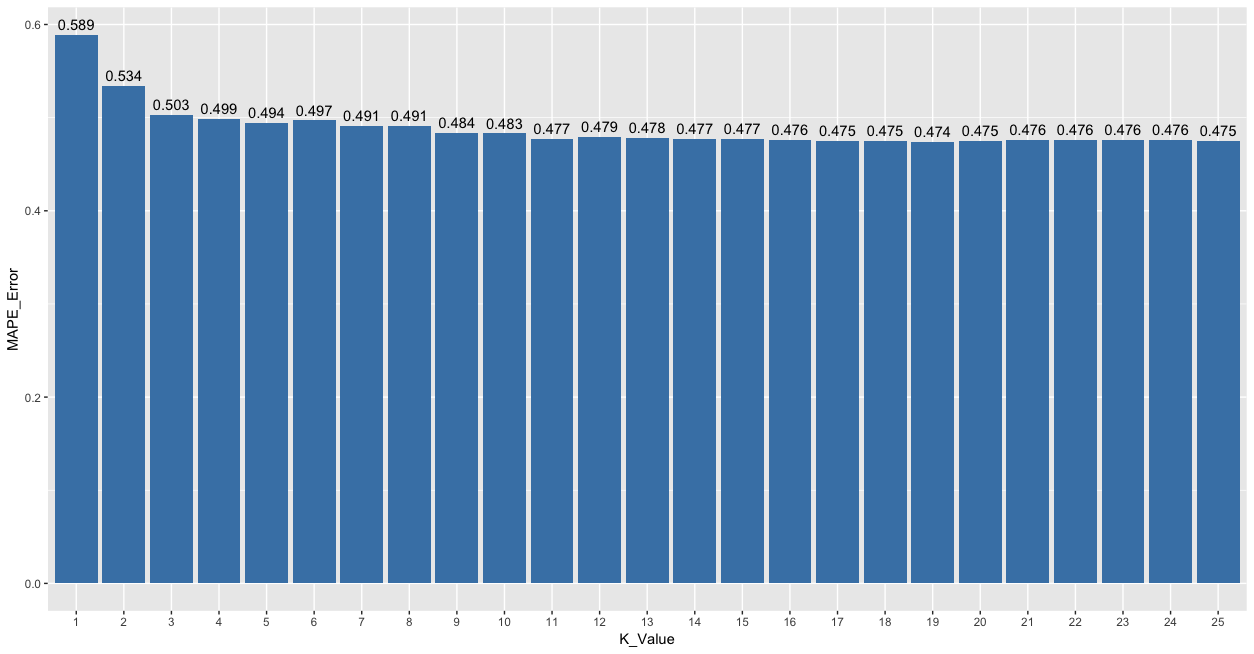
\includegraphics[scale=0.25]{Mean-MAPE.png}

For MAPE, we see the error decrease as we increase the k value. This is expected because initially, the more the nearest neighbours, intuitively, the more accurate the prediction.

For mean results tested against PGEC accuracy:

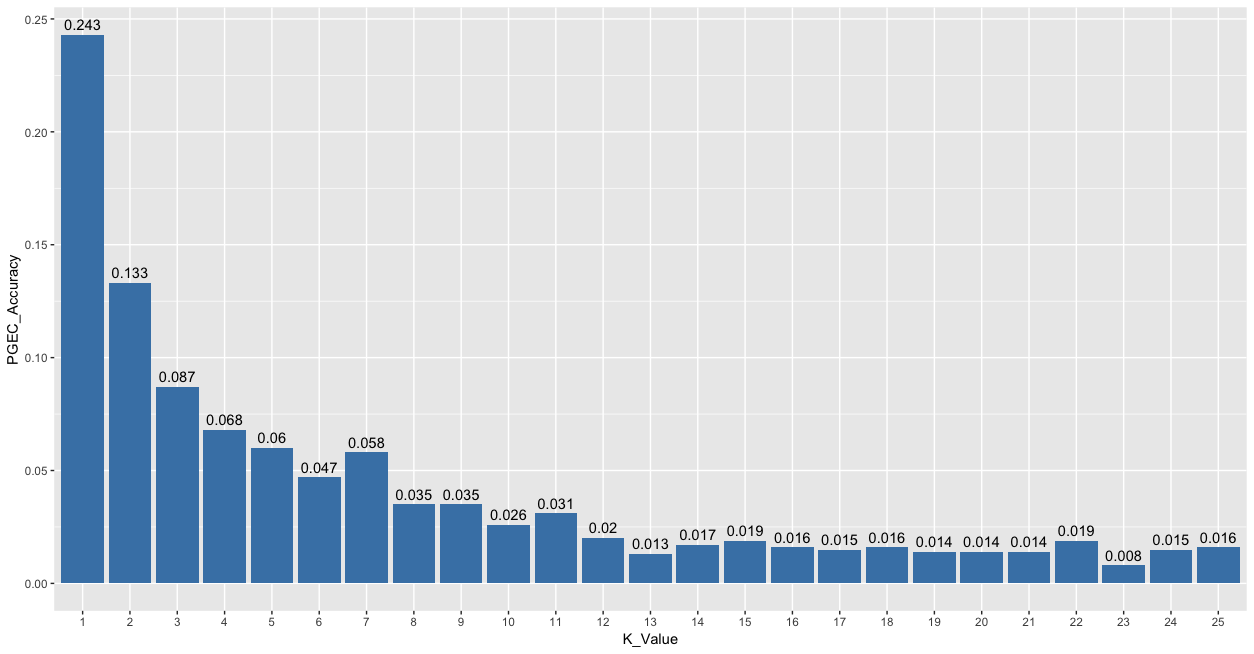
\includegraphics[scale=0.25]{Mean-PGEC.png}

We can see that there is a general decrease in PGEC accuracy as the k value tested increases. If we look closely at the datasets we can reason that this is because most of the ratings are integers. More nearest neighbours means higher probability of decimal. Because of this we cannot conclude from this graph that there was a decrease in accuracy since it was affected by the nature of the way the ratings were made. We can also therefore conclude that PGEC does not describe the error to the fullest extent

For median results tested against MAPE error:

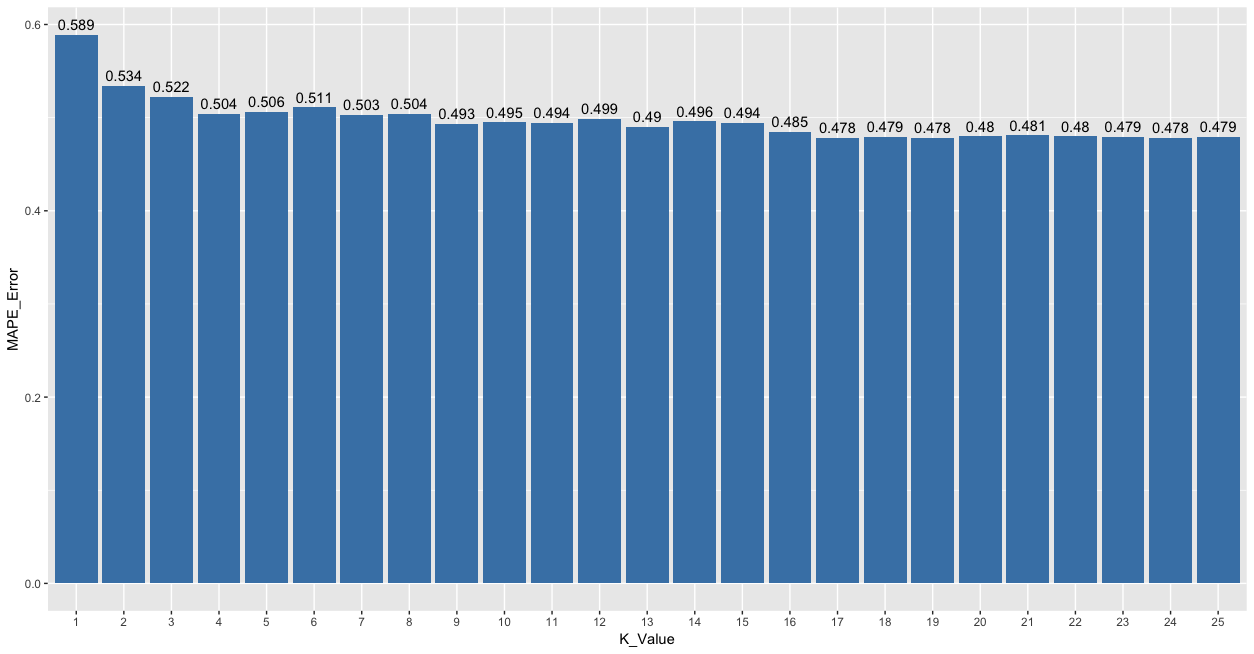
\includegraphics[scale=0.25]{Median-MAPE.png}

Similar to the results for mean, we can see that the MAPE error decreases as the k value increases. This is expected because intuitively the more neighbours we source, the more accurate the prediction

For median results tested against PGEC accuracy:

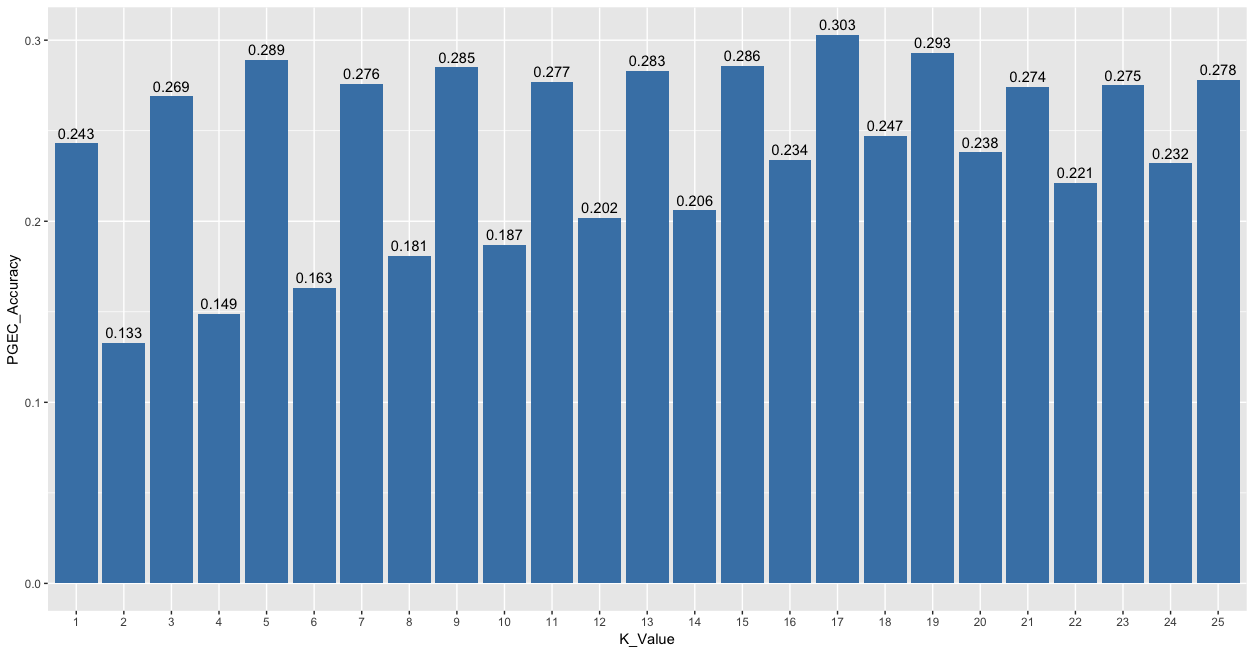
\includegraphics[scale=0.25]{Median-PGEC.png}

We can observe three things from this graph. The first is that when k is even, the accuracy is significantly lower than nearby k value results. This is because of the way median is calculated (where the middle two neighbours' ratings are averaged, so there is a high probability of getting a decimal value from adding an odd and an even value). The second thing we can observe from this graph is that there is a general increase in accuracy as k increases where k is even. This expected because as k increases, the rating is more representative of the user's preferences. The third thing we can gather from this graph is that there is a weak increase in accuracy as k increases where k is odd. However, because the values fluctuate, we cannot conclude anything significant from this weak trend. 

For mode results tested against MAPE error:

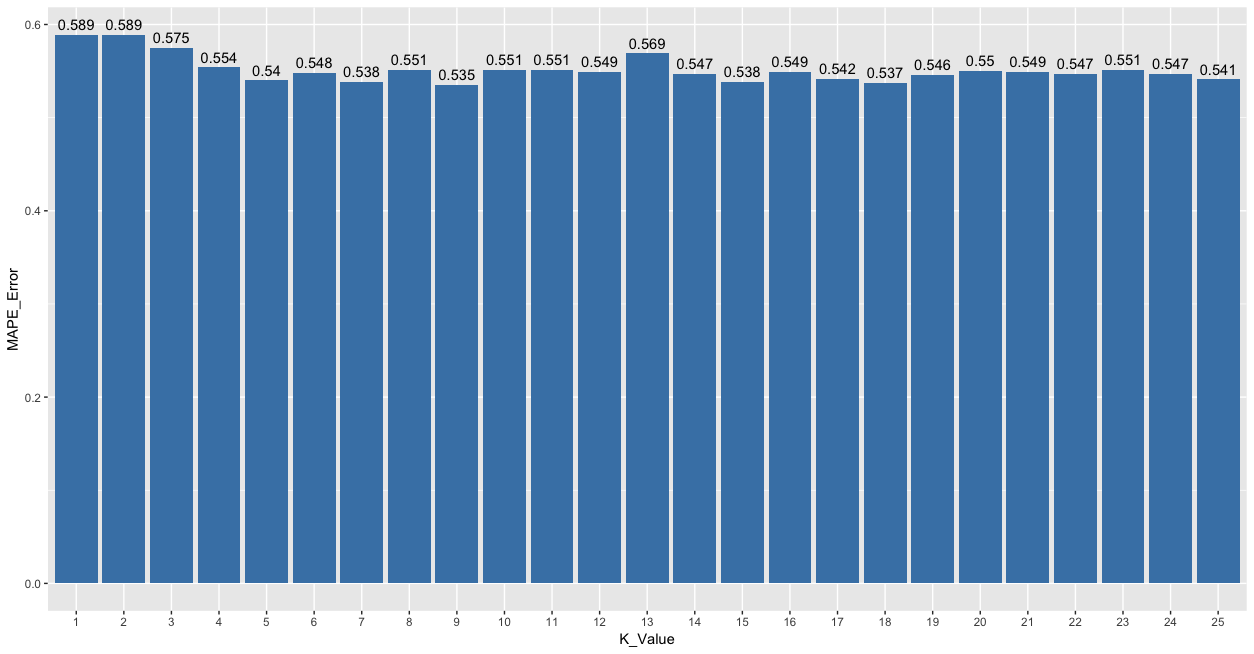
\includegraphics[scale=0.25]{Vecmode-MAPE.png}

We can observe that there is a general decrease in the MAPE error as k value increases at the beginning. This is expected, but we cannot conclude anything significant as k increases further because the MAPE error values fluctuate. However, we can predict that this is because statistically the statistical value of mode diminishes as there are more neighbours since they are less representative of the user. 

For mode results tested against PGEC accuracy:

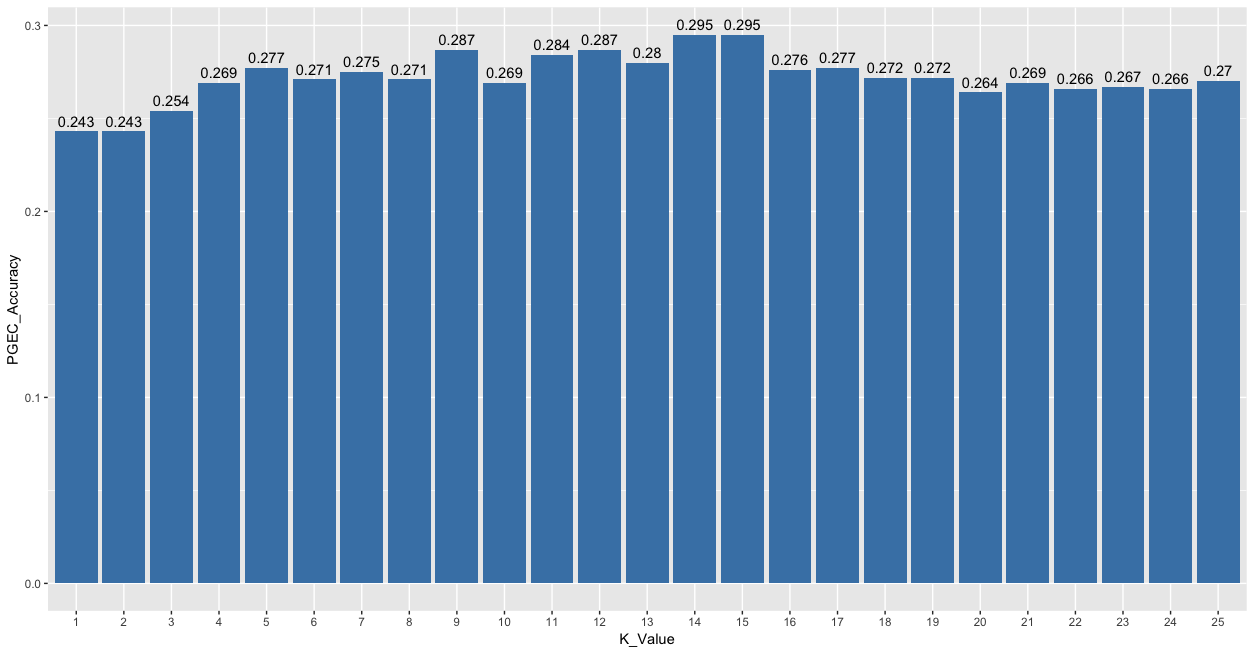
\includegraphics[scale=0.25]{Vecmode-PGEC.png}

We can observe that the accuracy increases before decreasing. The reasoning similar to that of the MAPE error graph. Initially, as k increases (in the range of 10 to 13), they become more representative of the user's choices, but as it increases further, the extra users that are maybe not so close to the user affects the accuracy, thus bringing it down and making the final result less representative of the user's choices. Perhaps this is an indicator of the best choice of number of neighbours to be used in this dataset.

\section{Evaluation}
For MAPE error indicators, there is a somewhat larger error for the vecmode results as compared to the results for mean and median. Perhaps this is an indicator that vecmode is not as suitable for prediction as mean and median in predicting these ratings. For PGEC error indicators, we found that mean does not do as well as the other local measures, which is expected due to the nature of the ratings (being mostly integers and mean giving mostly decimals).


\end{document}